\chapter{Vergleich}
\section{Testumgebung}
Für den Vergleich der beiden API Ansätze wurde eine Single-Page Anwendung mit dem Vue.js Framework als Client und jeweils eine REST API und GraphQL API mit der Node.js Serverlaufzeitumgebung entwickelt.
Als Datenquelle dient zum einen eine MongoDB Datenbank, sowie Dateien im JSON Format.
Durch die Verteilung der jeweiligen Softwarekomponenten auf physikalisch unterschiedliche Rechner, lassen sich mehrere Anwendungsfälle abbilden.
So wurden die Clientanwendung, die Serveranwendungen und die Datenbank in verschiedenen Kombinationen lokal und von Cloudumgebungen (Azure, Heroku, MongoDB Atlas) gehostet und ausgeführt.
Die JSON Dateien als Alternative zur Datenbank ermöglichen es das Kontingent der Clouddatenbank nicht unnötig zu belasten und den durch Datenbankabfragen entstehenden Overhead auf die deutlich schnellere Dateilesezeit zu minimieren.
Bei den Messungen wurde auf das Angleichen der Testbedingungen geachtet, besonders die im Zusammenhang mit Clouddiensten gemessenen Werte sind jedoch stark von der je nach Tageszeit unterschiedlichen, unbekannten Belastung des Dienstes abhängig.
\begin{figure}[h]
  \centering
  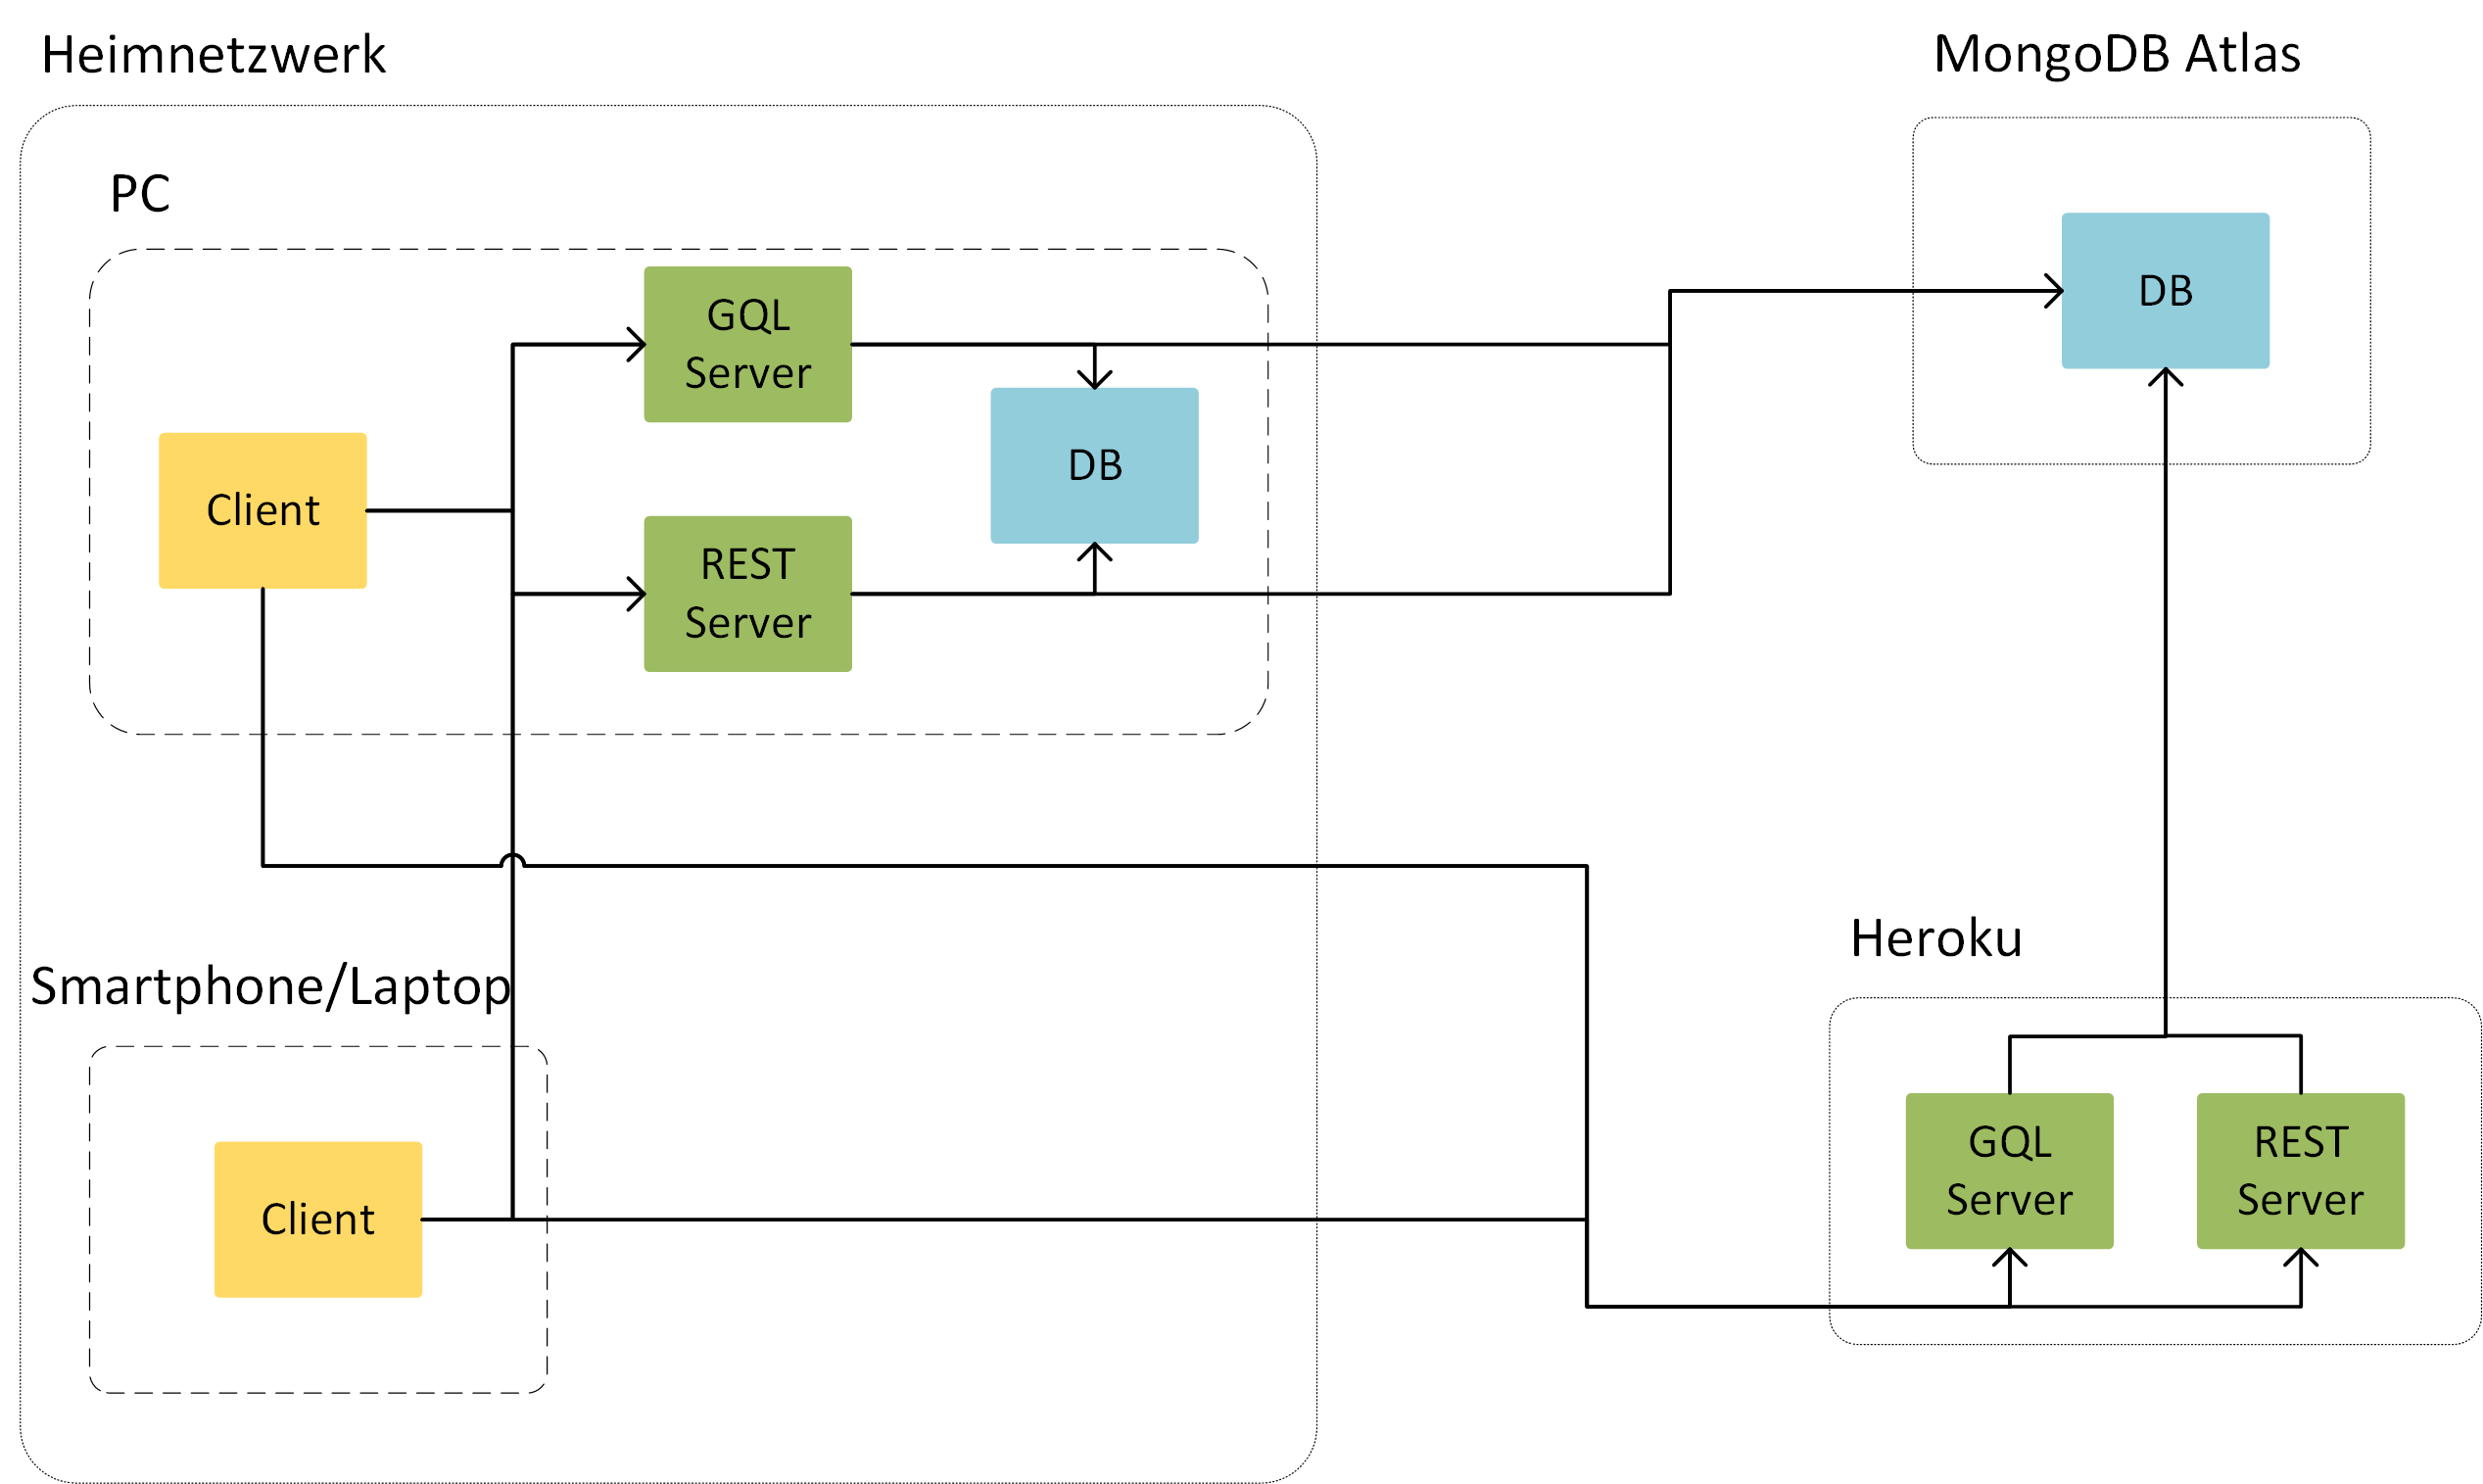
\includegraphics[width=\linewidth]{../Kapitel/Grafiken/netzwerk.png}
  \caption{Testumgebung}
  \label{img:REST-diss}
\end{figure}
\section{Abfrageflexibilität}
\begin{itemize}
  \item GraphQL
  \begin{itemize}
    \item unterscheidet Feldselektion, Sortieren, Filtern, Optionen
    \item keine Syntax für Sortieren/Filtern, aber Möglichkeit über Feldargumente
    \item Bsp: height (unit:FOOT)
    \item an Query sind Performanceprobleme evtl.\ schwer erkennbar (siehe Tools)
  \end{itemize}
  \item REST
  \begin{itemize}
    \item fields=`` '' für Feldselektion
    \item field=`` '' zum Filtern
    \item sort=[field],sort-dir=desc zum Sortieren
    \item option=`` '' für Optionen
    \item includes empfohlen bei JSON:API, aufbrechen von HATEOAS\@?
  \end{itemize}
  \item Upload ist schwierig für GraphQL (serialization), REST kann multipart/form-data header nutzen
\end{itemize}
Bei der Entwicklung von Client-Anwendungen ist die Flexibilität der genutzten API ein entscheidender Einflussfaktor.
Dabei steht meistens die Flexibilität für das Generieren der Abfragen zum Empfangen von Daten im Vordergrund, aber auch Operationen zum Modifizieren von Ressourcen müssen betrachtet werden.
\par
GraphQL wurde als Abfragesprache entwickelt.
Eines der Entwicklungsziele ist es, dass eine Clientanwendung mit einer einzigen Abfrage alle für eine Ansicht nötigen Daten erhalten kann.
Der Server gewährt Zugriff auf das Datenschema, welches alle verfügbaren Daten und deren Relationen darstellt, sowie die Einstiegspunkte (Root Query), auf deren Basis ein Client seine Anfrage aufbauen kann.
Das Schema stellt den Rahmen für alle Abfragen dar.
Alle Daten, die der Server zur Verfügung stellt, werden durch Typen und deren Felder repräsentiert.
Jedes Feld, welches eine Clientanwendung erhalten möchte, muss in der Query angegeben werden.
Es existiert keine Möglichkeit alle Felder eines Typs zu erhalten ohne jedes davon anzugeben, \zB{} durch Wildcard Zeichen.
Der Client ist damit eng an das Schema gekoppelt, erhält aber auch nur die Daten, die tatsächlich angefragt wurden.
Die Möglichkeit eines GraphQL-Servers beliebige Abfragen innerhalb des Schemas auszuwerten eignet sich besonders für öffentliche APIs, bei denen dem API-Entwickler die individuellen Anforderungen und damit die Abfragen verschiedenster Anwendungen, im Voraus nicht bekannt sind.
Die Relationen zwischen den Datentypen werden durch das Schema festgelegt.
Eine Anfrage kann jedoch beliebig viele, unabhängige Queries beinhalten, \zB{} um verschiedene Daten zu erhalten, die in keiner Beziehung zueinander stehen oder deren Beziehung durch das Schema nicht dargestellt wird.
Der Server kann für jedes Feld Parameter anbieten, welche die Auswertung des Feldwertes verändern. Über solche Feldargumente können Optionen, die Geschäftslogik darstellen, aber auch allgemeine Abfragefunktionen, wie \zB{} Sortieren und Filtern zur Verfügung gestellt werden.
Einem Feld \enquote{Breite} könnte beispielsweise die Maßeinheit als Option übergeben werden.
\par
Während das Anfragen von Daten sehr viel Flexibilität für Clients bietet, ist das Modifizieren von Ressourcen nach Konvention nur über einzelne Mutations möglich.
Üblicherweise wird für jede Operation (Erstellen, Verändern und Löschen) einer Ressource eine separate Mutation zur Verfügung gestellt, welche durch den Namen eindeutig identifiziert wird.
Die Antwort auf eine Mutation kann wieder ein Objekt sein und genutzt werden um das Resultat der Operation zu übermitteln oder den neuen Stand der Ressource abzufragen.
\par

In einer REST API ist jede Ressource über einen separaten Endpunkt erreichbar.
Das Veröffentlichen einer neuen Ressource geschieht durch das Einführen eines neuen Endpunktes.
Ein Endpunkt kann alle Methoden zum Abfragen und Ändern einer Ressource bereitstellen und durch die HTTP Verben semantisch unterscheiden.
Die Antwort auf einen GET Request an einen Endpunkt enthält alle Felder der Ressource bzw.\ die komplette Repräsentation.
In Beziehung stehende Daten, die nicht Teil einer Ressource sind, müssen über mehrere Requests vom Server angefragt werden.
Der Grundgedanke von HATEOAS ist, dass diese verbundenen Ressourcen Verweise aufeinander enthalten, wodurch ihre Beziehung dargestellt wird.
Das Zusammenbauen von Requests anhand der Links in erhaltenen Ressourcen ermöglicht große Flexibilität, erfordert jedoch dass Daten erst ausgewertet werden müssen und danach erst neue Anfragen abgesetzt werden können.
Dadurch ist das Datenmodell nicht durch ein Schema vorgegeben, sondern kann zur Laufzeit geändert und explorativ genutzt werden, da es selbstdokumentierend ist.
Oftmals ist bei der Entwicklung von Clientanwendungen die erforderliche Datenstruktur jedoch bekannt und ist es wünschenswert möglichst alle benötigten Informationen von wenigen Endpunkten zu erhalten, um die Performance zu steigern.
Dazu gibt es verschiedene Ansätze, wie der Query-String einer URI genutzt werden kann, um in Beziehung stehende Daten mit einem einzigen Request von einem Endpunkt zu erhalten.
Weder REST noch HTTP spezifizieren Syntax und Semantik des Query Strings bzw.\ betrachten diese als Implementierungsdetail.
Query-Parameter und Matrixparameter werden häufig gebraucht, um die Möglichkeiten von Abfragesprachen für REST zu implementieren.
Sie ermöglichen \zB{} die gewünschten Felder des angefragten Objektes, ein Feld nach dem sortiert, oder ein Feld und Wert nach dem gefiltert werden soll, anzugeben.
Somit können Clientanwendungen die Antwort je nach ihren Anforderungen besser beeinflussen.
Abhängig davon wie unterschiedlich diese sind, muss die Entscheidung über die Erweiterung der Parameteroptionen oder das Einführen eines separaten Endpunktes getroffen werden.
Über sogenannte \enquote{includes} lassen sich bei JSON:API verbundene Objekte in die Antwort einbeziehen.
Includes oder sind außerdem eine effektive Lösung für das N+1 Problem.
Diese speziellen Auswertungen des Query-Strings müssen durch den REST Server angeboten werden und sind aus Entwurfssicht ein Tausch von erhöhter Abfragekomplexität und Clientflexibilität gegen Serverperformance.
\par
Da GraphQL für die Übertragung von Daten in Textform konzipiert wurde, müssen Informationen als Text vorliegen, oder serialisiert werden.
Das kann besonders beim Hochladen von Binärdaten, wie Audio- oder Videodateien, zu sehr großen Datenmengen führen.
Eine REST API kann Binärdaten mit dem MediaType \enquote{multipart/form-data} empfangen und verarbeiten.
Für eine GraphQL API muss entweder ein Dateiupload-Service vorgeschaltet sein und nur der Link übertragen, oder eine Bibliothek, wie \enquote{graphql-upload}, verwendet werden.

\section{Weiterentwicklung und Versionierung}
\begin{itemize}
  \item GraphQL
  \begin{itemize}
    \item neue Felder hinzufügen ohne existierende Queries zu beeinflussen
    \item neue Felder nicht automatisch gesendet
    \item Felder als deprecated markieren → Tool kann Entwickler warnen
    \item Monitoring auf Feldlevel möglich
  \end{itemize}
  \item REST
  \begin{itemize}
    \item Monitoring: werden sparse fieldsets oder includes verwendet können genutzte Felder aufgezeichnet werden
    \item neue Version, neuer Endpunkt example.com/v2/contacts/\dots
    \item für kleine Veränderungen ungeeignet
    \item Hinzufügen von Ressourcen → keine Versionierung notwendig
    \item Semantische Versionierung
    \item Postelsches Gesetz
    \item Hinzufügen/Umordnen von einzelnen Elementen sollte Client akzeptieren
    \item Versionierung über Accept-Header, URI oder query string
  \end{itemize}
\end{itemize}
\par 
Langlebige Software befindet sich in ständiger Entwicklung.
Ein Server muss auf Veränderungen des der API zugrunde liegenden Datenmodells reagieren können und diese gegebenenfalls Clients zugänglich machen.
Neue Anforderungen an die API erfordern das Erweitern der Abfragemöglichkeiten, oder das Verringern derselben, wenn alte Funktionalität nicht mehr unterstützt oder durch neue ersetzt werden soll.
Da jede API einen Vertrag zwischen Server und Client darstellt, sollten Veränderungen einem festgelegten Ablauf und Kommunikationskanal folgen, um sukzessive Migration zu gewährleisten und Abfragefehler zu vermeiden.
Zu diesem Zweck wird in der Softwareentwicklung häufig Versionierung verwendet, bei der durch eine Zahl oder Zahlenkombination ein bestimmter Stand der Software bereitgestellt oder abgefragt wird.
\par
Um eine REST API um zusätzliche Ressourcen zu erweitern, ist keine Versionierung notwendig.
Stattdessen wird ein neuer Endpunkt hinzugefügt und über die Verlinkung von anderen Ressourcen, oder als Einstiegspunkt in der Dokumentation bekanntgemacht.
Eine API Clientanwendung sollte so entwickelt werden, dass eine Antwort ausgewertet werden kann, solange sie semantisch eindeutig verständlich ist (Postel'sches Gesetz).
Das Umordnen und Hinzufügen von Elementen innerhalb einer Antwort sollte somit nicht zu Fehlern führen und die Validierung demgegenüber tolerant sein.
Normalerweise muss erst versioniert werden, wenn keine Rückwärtskompatibilität mehr gewährleistet werden kann.
Eine neue Version einer Ressource kann über mehrere Wege bereitgestellt und angefragt werden.
\begin{enumerate}
  \item Jeder Request kann einen Accept-Header enthalten, der zur Identifikation der zu sendenden Repräsentation genutzt werden kann.
  Sendet ein Client \zB{} einen Accept-Header mit dem Wert application/vnd.format.v2+json, so kann der Server durch Content-Negotiation anhand des \enquote{v2} die zu sendende Version ermitteln.
  \item Die URI als Identifikationsmittel kann ebenfalls genutzt werden, um verschiedene Versionen einer Ressource kenntlich zu machen.
  Die Anfrage an example.com/v2/events entspricht dem Erstellen eines neuen Endpunktes.
  Der Server muss nun auf einem weiteren Endpunkt antworten können, die Komplexität jedes einzelnen Endpunktes wird jedoch nicht erhöht.
  \item Für kleine Änderungen, wie das Ändern oder Entfernen eines einzelnen Feldes, ist normalerweise kein neuer Endpunkt nötig.
  Würde für jede dieser verhältnismäßig kleinen Änderungen ein neuer Endpunkt erstellt werden, ginge schnell die Übersichtlichkeit über die Menge der Endpunkte und deren Unterschiede verloren.
  Die URI der Ressource kann für verschiedene Versionen genutzt werden und stattdessen die Versionsinformationen im Query String transportiert werden (\zB{} example.com/events?version=2).
  Diese Variante teilt den gleichen Nachteil, den alle Query String Optionen haben, dass der Serverhandler für diesen Endpunkt komplexer und die Performance verringert wird.
  Es ist denkbar, dass nicht nur jede einzelne Option geprüft werden muss, sondern dass die Option für die Version der Ressource auch Auswirkung auf andere Optionen hat, sodass der Server einen Entscheidungsbaum auswerten muss, bevor eine Antwort gesendet werden kann.
\end{enumerate}
Wurde eine neue Version einer Ressource zur Verfügung gestellt, muss diese auch erreichbar sein.
Da die Änderungen von Variante 2 und 3 sich allein auf die URI auswirken, müssen in verknüpften Ressourcen die Links zur neuen Version aktualisiert werden.
Da Header in einem Link nicht repräsentiert werden können, ist es bei der ersten Variante notwendig, dass der Client über die neue Version informiert wird und allen Anfragen an die Ressource den Accept-Header hinzufügt.
\par
Beim Entfernen von Funktionalität ist es sinnvoll die aktuelle Nutzung derselben durch Monitoring festzustellen und notwendig die geplanten Änderungen zu kommunizieren.
Da normalerweise die gesamte Repräsentation einer Ressource als Antwort gesendet wird, kann nur die Nutzung des Endpunktes und nicht die tatsächliche Notwendigkeit einzelner Teile der Ressource bzw.\ Felder ermittelt werden.
Das ist jedoch möglich, wenn bei jeder Anfrage mittels Includes die gewünschten Felder angegeben werden müssen.
Sollen einzelne Elemente einer Ressource nicht mehr gesendet werden, so können diese zeitweise den für den Datentyp üblichen Nullwert enthalten, bevor sie endgültig entfernt werden.
Wird ein Endpunkt der API entfernt, so sollte der Server mit dem entsprechenden HTTP Status Code (410 Gone) antworten und alle Links in verknüpften Ressourcen müssen gelöscht werden.
Ist eine Ressource lediglich unter einem anderen Endpunkt erreichbar, so kann der Code 310 \enquote{Moved Permanently} den Client automatisch zur neuen URI weiterleiten.
\par
Erklärtes Ziel von GraphQL ist es Versionierung zu verhindern und stattdessen die API kontinuierlich, abwärtskompatibel weiterzuentwickeln.
Da jedes Feld, welches ein Client erhalten möchte, in der Query explizit angegeben werden muss, ist detailreiches Monitoring bis auf Feldebene möglich.
Im Datenmodell neu eingeführte Felder beeinflussen bestehende Abfragen nicht, können aber jederzeit in diese aufgenommen werden.
Felder, die zukünftig aus der API entfernt werden sollen, können mit isDeprecated als veraltet gekennzeichnet und ein Grund als Metainformation angegeben werden.
Diese Kennzeichnung beeinflusst die Abfrage des Feldes nicht, kann aber per Introspektion zur Entwicklungszeit von Tools abgefragt und dem Entwickler als Warnung angezeigt werden.
Enthält eine Abfrage Felder, die im Schema nicht mehr enthalten sind, schlägt die Abfrage fehl.
Änderungen in der Auswertungslogik einzelner Felder können über optionale Feldargumente bereitgestellt werden.
Auch diese beeinflussen bestehende Abfragen ohne diese Argumente nicht.
Für Feldargumente und Input Typen existiert zur Zeit noch keine Möglichkeit diese als veraltet zu kennzeichnen, ist aber für den nächsten Release der GraphQL Spezifikation geplant.
Ein GraphQL Server stellt ein Schema und damit alle darin enthaltenen Abfragen unter einer URI bereit.
Ergibt sich die Notwendigkeit eine neue Version unter einer anderen URI zu veröffentlichen, so können Abfragen die Schemata nicht verbinden und werden vom Server nur im Kontext eines Schemas ausgewertet.
\section{Performance}
Zum Vergleich der Abfrageperformance von GraphQL und REST wurden jeweils nacheinander eine Reihe von Abfragen durchgeführt und gemessen, um die Charakteristik der Daten zu erforschen.
Die kostenfreie Laufzeitumgebung von Heroku (Dyno) unterliegt einem monatlichen Stundenlimit und wird nach 30 Minuten, in denen keine Anfragen gestellt werden, in den Schlafzustand versetzt.
Erhält eine schlafende Dyno eine Anfrage, so wird sie nach einer kurzen Verzögerung wieder aktiv. TODO Zitat Heroku
Diese anfängliche Verzögerungszeit ist nach der angegebenen 30 minütigen Pause, in geringerem Maße aber auch nach nur wenigen Sekunden Inaktivität zu beobachten.\ref{img:abfrage-zeitverlauf}
Diese anfänglichen Ausreißer sind unabhängig von der verwendeten API, wurden aber aufgrund der hohen Schwankungen in den weiteren Untersuchungen nicht einbezogen. 
\begin{figure}[h!]
  \centering
  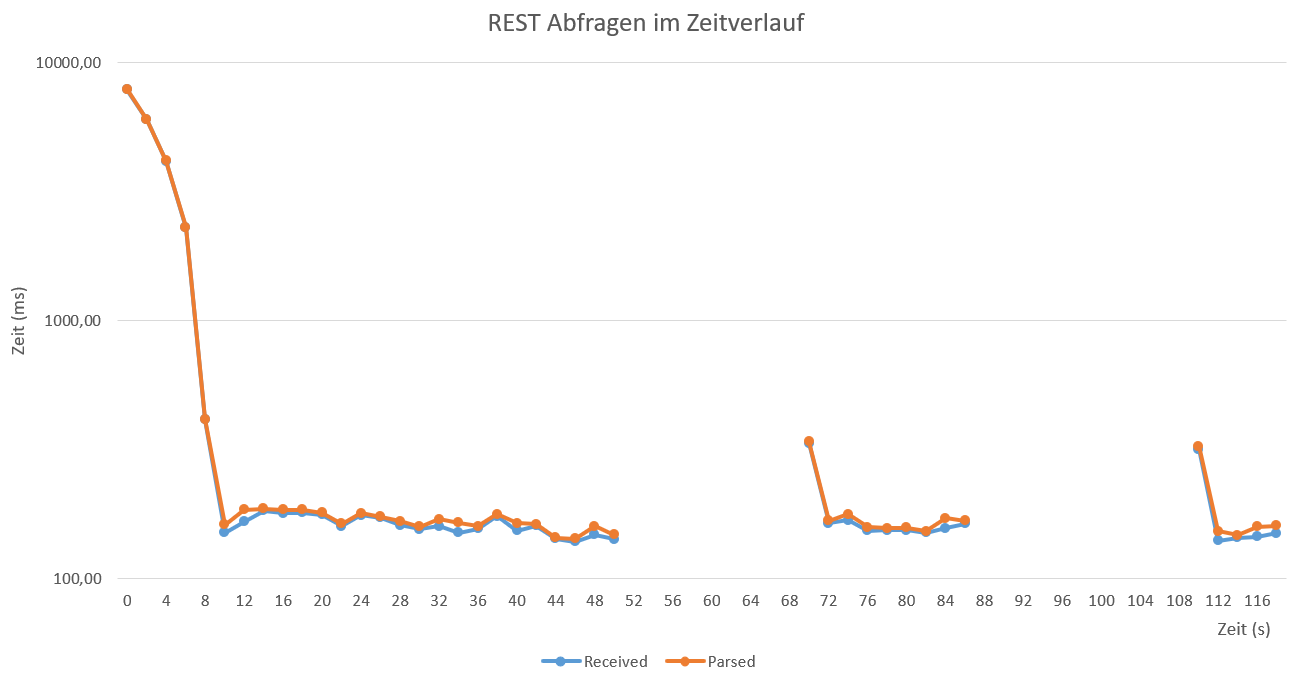
\includegraphics[width=\linewidth]{../Kapitel/Grafiken/abfragen-zeitverlauf.png}
  \caption{Abfragen im Zeitverlauf}
  \label{img:abfrage-zeitverlauf}
\end{figure}
Je nach für die Abfrage verwendetem Gerät unterscheiden sich die Abfragezeiten deutlich.
\begin{figure}[h!]
  \centering
  \includegraphics[width=\linewidth]{../Kapitel/Grafiken/abfrage-gerät.png}
  \caption{Abfragen nach Gerät}
  \label{img:abfrage-gerät}
\end{figure}
\begin{figure}[h!]
  \centering
  \includegraphics[width=\linewidth]{../Kapitel/Grafiken/parsing-gerät.png}
  \caption{Testumgebung}
  \label{img:REST-diss}
\end{figure}
\begin{figure}[h!]
  \centering
  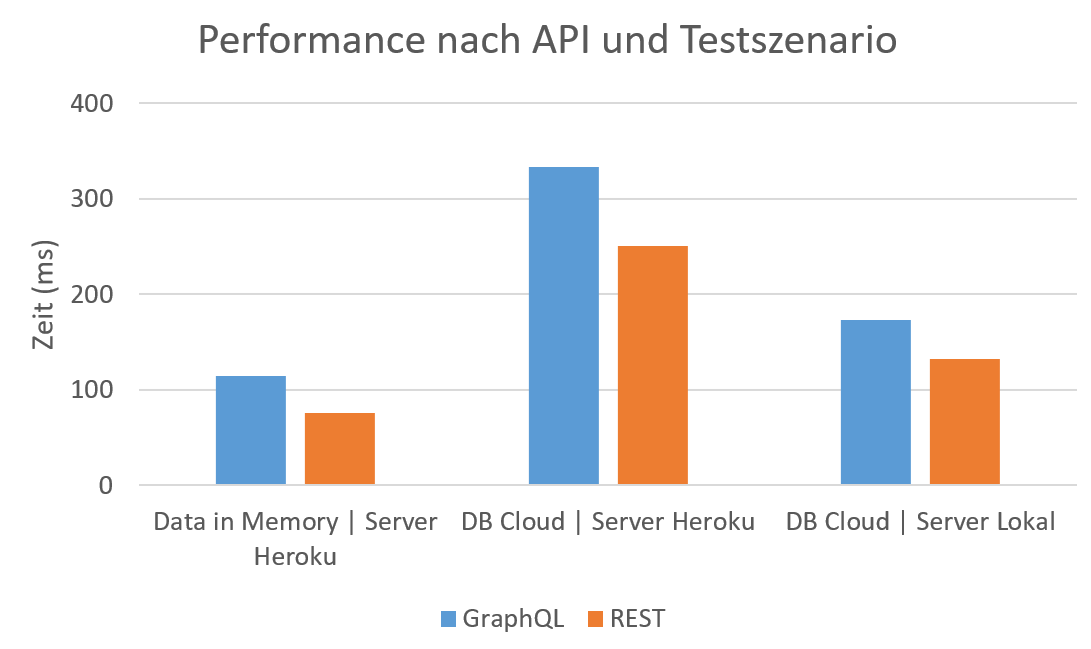
\includegraphics[width=\linewidth]{../Kapitel/Grafiken/performance-szenario.png}
  \caption{Testumgebung}
  \label{img:REST-diss}
\end{figure}
\begin{figure}[h!]
  \centering
  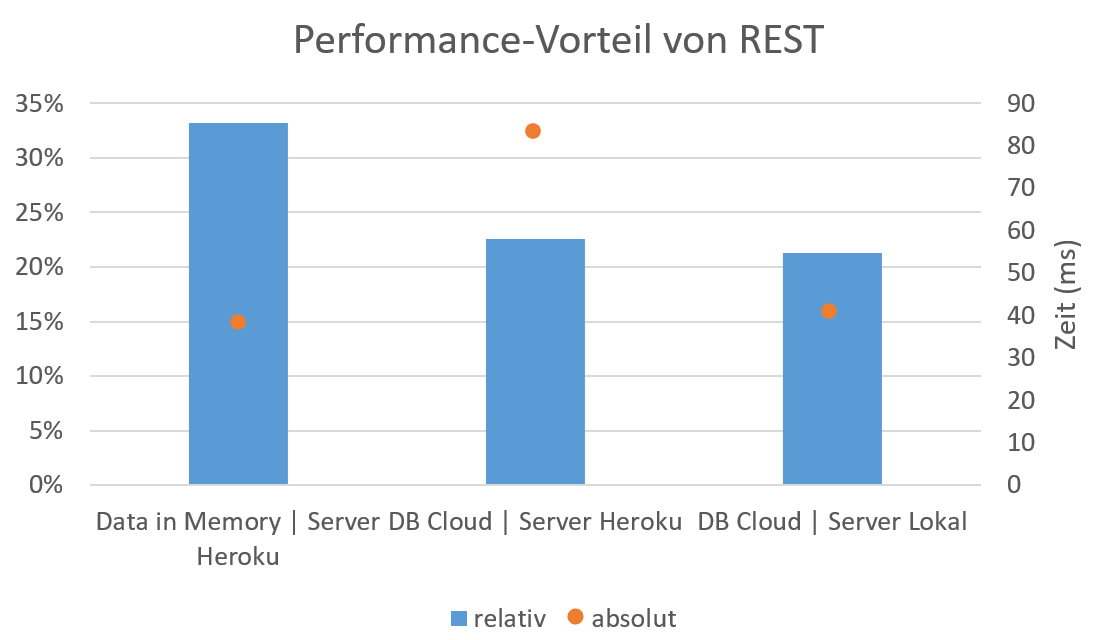
\includegraphics[width=\linewidth]{../Kapitel/Grafiken/performance-diff.png}
  \caption{Testumgebung}
  \label{img:REST-diss}
\end{figure}

\section{Datenaufkommen/Netzwerklast}
\begin{itemize}
  \item Transfer, Verarbeiten und Speichern unnötiger Daten (Felder) sollte vermieden werden
  \item GraphQL
  \begin{itemize}
    \item automatisch kleinstmöglicher Request
    \item Query muss an Server gesendet werden
  \end{itemize}
  \item REST
  \begin{itemize}
    \item standardmäßig gesamte Repräsentation
    \item viele APIs bieten Feldselektion an (Partials)
    \item query string enthält Feldselektion nach bestimmter Syntax
    \item je komplexer, desto mehr Daten
    \item jede Ressource ist extra Endpunkt
    \item für mehrere Ressourcen müssen mehrere Requests gemacht werden, n+1 Problem
    \item includes beziehen verbundene Daten in Response ein → ein Request für mehrere Ressourcen
  \end{itemize}
  \item GraphQL und REST Partials unterscheiden Objekt und Array nicht → Wissen über API notwendig um Performance einzuschätzen
  \item mehr Daten um Request genauer zu machen, sinnvoll um deutlich weniger Daten als Response zu erhalten
\end{itemize}

\section{Caching}
\begin{itemize}
  \item Flexibilität gegen Caching: je spezieller die Abfrage, desto schwieriger (weniger sinnvoll) caching
  \item nicht Antwort direkt cachen (HTTP), sondern manuell Objekte anhand ID cachen (JavaScript)
  \item REST
  \begin{itemize}
    \item Browser HTTP caching automatisch genutzt
    \item Caching basierend auf Endpunkt
    \item URL ist cache ID für die Ressource
    \item ermöglicht HTTP cache proxies
    \item je spezieller der query string, desto weniger cache Treffer
  \end{itemize}
  \item GraphQL
  \begin{itemize}
    \item POST response wird normalerweise nicht gecacht
    \item standardmäßig keine ID für caching vorhanden. Empfehlung: API sollte ID pro Objekt bereitstellen
  \end{itemize}
\end{itemize}

\section{Batching/Deduping}
\begin{itemize}
  \item GraphQL queries können parallel ausgewertet werden, Mutations nicht
\end{itemize}

\section{Fehlerbehandlung}

\section{Sicherheit}

\section{Kosten}

\section{Lernkurve, Fehlersuche, Community}

\section{Bibliotheken und Tools}
\begin{itemize}
  \item GraphQL
  \begin{itemize}
    \item offizielle Spezifikation vorhanden
    \item Referenzimplementierung in JavaScript
    \item Zusatztools von Facebook (Dataloader, Relay)
    \item Tool kann Abfragekomplexität zu Entwicklungszeit ermitteln (mit vergangenen Messwerten)
  \end{itemize}
\end{itemize}
